\batchmode
\documentclass[fleqn]{beamer}

\usepackage{graphicx}
\graphicspath{{figures/}}

\usepackage[dvipsnames]{xcolor}
\definecolor{keywordorange}{RGB}{214, 109, 17}
\definecolor{darkgreen}{RGB}{15, 150, 15}
\definecolor{darkblue}{RGB}{0, 0, 180}
\newcommand{\registergrey}{gray!25}

\usepackage{tikz}
\usepackage{tikz-timing}
\usetikzlibrary{fit, positioning, shapes.geometric, shapes.symbols}
\tikzset{
    node distance=1em and 3em,
    blk/.style={ draw=black, very thick },
    % Functional unit
    fu/.style={ blk, rectangle, inner sep=0.5em },
    % Register
    reg/.style={ fu, fill=\registergrey },
    clk/.style={ isosceles triangle, isosceles triangle apex angle=80, draw=black, very thick, anchor=right corner, scale=0.33 },
    adder/.style={ blk, circle, inner sep=0.2em },
    line/.style={ black, very thick },
    arrow/.style={ line, -> },
}
\newcommand{\clkx}{0.2mm}
\newcommand{\clky}{0.5mm}

\usepackage{lstautogobble}
\usepackage{listings}
\lstdefinestyle{irstyle}{
    basicstyle=\scriptsize\ttfamily,
    language=c,
    commentstyle={\color{gray}},
    frame=tb,
    tabsize=2,
    keywords=[1]{
        sbuild, sdata, letstm, let, in, vbuild, true, false,
        const, accelerator, assert, yields,
        default, undefined, truncate18,
        StmMap, StmReduce, StmZip, StmSum, StmSlideInit, VecAll, MulAddCascaded, StmCst
    },
    keywordstyle=[1]{\color{darkblue}\bfseries},
    morekeywords=[2]{init, next, stm, ready, if, then, else},
    keywordstyle=[2]{\color{darkgreen}\bfseries},
    emph={bool, u4, u8, u16, u32, i8, i16, i18, i32, fix8_7, Vec, Stm, ->},
    emphstyle={\color{keywordorange}\bfseries},
    mathescape=true,
    numberstyle={\color{gray}},
    autogobble=true,
    escapeinside={<@}{@>}
}
\lstset{style=irstyle}

\usepackage{xspace}
\usepackage{siunitx}
\usepackage{booktabs}

\usepackage{pifont}
\newcommand{\mycheckmark}{\ding{52}}
\newcommand{\mycrossmark}{\ding{56}}

\usepackage{hyperref}
\hypersetup{
    colorlinks=true,
    urlcolor=blue,
    linkcolor=.
}
\newcommand{\dspmergerequest}{\href{https://gitlab.cern.ch/atlas-lar-be-firmware/LASP/LASP-dacore/-/merge_requests/143}{!143}\xspace}
\newcommand{\validmergerequest}{\href{https://gitlab.cern.ch/atlas-lar-be-firmware/LASP/LASP-dacore/-/merge_requests/142}{!142}\xspace}
\newcommand{\dsppackingpresentation}{\url{https://indico.cern.ch/event/1700332/}\xspace}

\usetheme{Berlin}
\usecolortheme{beaver}
\title{\ourlang{}: High-Level Synthesis with Parallel Patterns}
\author{\underline{Louis Hildebrand} \and Brigitte Vachon \and Christophe Dubach}
% TODO: update color theme's red to match McGill's red?
\institute{
\includegraphics[scale=0.8]{mcgill_logo.pdf}}
\date{September 22, 2026}

\beamertemplatenavigationsymbolsempty

% https://tex.stackexchange.com/a/83054
\makeatletter
\setbeamertemplate{footline}
{
  \leavevmode%
  \hbox{%
      \begin{beamercolorbox}[wd=.25\paperwidth,ht=2.25ex,dp=1ex,center]{author in head/foot}%
        LAr Week September 2026
      \end{beamercolorbox}%
      \begin{beamercolorbox}[wd=.54\paperwidth,ht=2.25ex,dp=1ex,center]{title in head/foot}%
        \usebeamerfont{title in head/foot}\insertshorttitle
      \end{beamercolorbox}%
      \begin{beamercolorbox}[wd=.2\paperwidth,ht=2.25ex,dp=1ex,center]{date in head/foot}%
        \insertframenumber{} / \inserttotalframenumber
      \end{beamercolorbox}
  }%
  \vskip0pt%
}
\makeatother

\setbeamercovered{transparent}

\renewcommand{\thefootnote}{\fnsymbol{footnote}}
% Source - https://tex.stackexchange.com/a/21745
% Posted by Stefan Kottwitz, modified by community.
% Retrieved 2026-05-28, License - CC BY-SA 3.0
\let\oldfootnotesize\footnotesize
\renewcommand*{\footnotesize}{\oldfootnotesize\scriptsize}

\newcommand{\ourlang}{\textsc{Sirop}\xspace}

\begin{document}

\begingroup
\setbeamertemplate{footline}{}
\begin{frame}[noframenumbering]
    \titlepage
\end{frame}
\endgroup

\section*{Recap}

\begin{frame}[fragile]{Recap: Project Goal}
    \begin{center}
        Goal: simplify the implementation of resource-efficient data processing (e.g., energy reconstruction algorithms) on FPGA

        \vspace{\baselineskip}

        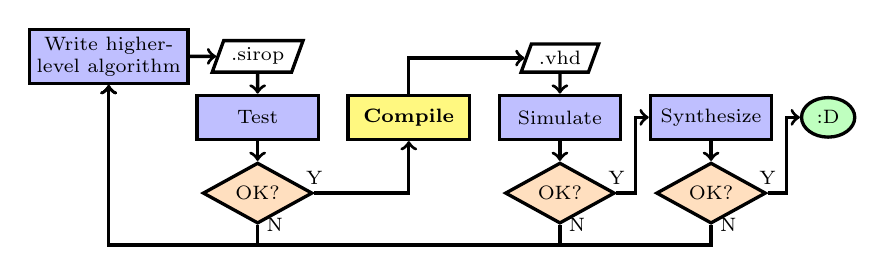
\begin{tikzpicture}[
            scale=0.5,
            node distance=0.9em and 1.2em,
            arrow/.style={->, black, very thick},
            flowchartnode/.style={draw, black, very thick, align=center},
            process/.style={flowchartnode, rectangle, fill=blue!25, minimum height=2em, minimum width=5.5em},
            hiprocess/.style={process, fill=yellow!50},
            decision/.style={flowchartnode, diamond, aspect=1.8, fill=orange!25},
            endpoint/.style={flowchartnode, ellipse, fill=green!25},
            io/.style={flowchartnode, trapezium, trapezium left angle=70, trapezium right angle=110}
        ]
            \scriptsize
            \node[process, align=center]                (write-sirop)       {Write higher-\\level algorithm};
            \node[io, right=of write-sirop]             (sirop-files)       {.sirop};
            \node[process, below=of sirop-files]        (run-sirop-tests)   {Test};
            \onslide+<1>
            \node[process, right=of run-sirop-tests]    (sirop-compile)     {Compile};
            \onslide+<2->
            \node[hiprocess, right=of run-sirop-tests]  (sirop-compile)     {\textbf{Compile}};
            \onslide+<1->
            \node[process, right=of sirop-compile]      (run-vsim)          {Simulate};
            \node[process, right=of run-vsim]           (synth)             {Synthesize};
            \node[endpoint, right=of synth]             (end)               {:D};
            \node[decision, below=of run-sirop-tests]   (sirop-tests-pass)  {OK?};
            \node[decision, below=of run-vsim]          (vsim-pass)         {OK?};
            \node[decision, below=of synth]             (synth-pass)        {OK?};
            \node[io, above=of run-vsim]                (vhdl-files)        {.vhd};
            \coordinate[below=of sirop-tests-pass]      (try-again);

            \draw[arrow] (write-sirop)      to (sirop-files);
            \draw[arrow] (sirop-files)      to (run-sirop-tests);
            \draw[arrow] (run-sirop-tests)  to (sirop-tests-pass);
            \draw[arrow] (sirop-compile)    |- (vhdl-files);
            \draw[arrow] (vhdl-files)       to (run-vsim);
            \draw[arrow] (run-vsim)         to (vsim-pass);
            \draw[arrow] (synth)            to (synth-pass);

            \draw[transparent] (run-vsim) to coordinate[midway] (sim-to-synth) (synth);
            \draw[transparent] (synth) to coordinate[midway] (synth-to-end) (end);
            \draw[arrow] (sirop-tests-pass) -| node[at start, above] {Y} (sirop-compile);
            \draw[arrow] (vsim-pass)        -| node[at start, above] {Y} (sim-to-synth) to (synth);
            \draw[arrow] (synth-pass)       -| node[at start, above] {Y} (synth-to-end) to (end);

            \draw[arrow] (sirop-tests-pass) |- node[at start, right] {N} (try-again) -| (write-sirop);
            \draw[arrow] (vsim-pass)        |- node[at start, right] {N} (try-again) -| (write-sirop);
            \draw[arrow] (synth-pass)       |- node[at start, right] {N} (try-again) -| (write-sirop);
        \end{tikzpicture}
    \end{center}

    \onslide<2->
    \begin{columns}[t]
        \scriptsize
        \newcommand{\regwidth}{1em}
        \newcommand{\regheight}{1.75em}
        \begin{column}{0.4\textwidth}
            \begin{center}
                \textbf{Latency matching} \\
                \begin{tikzpicture}[node distance=0em and 1.25em]
                    % Before latency matching
                    \onslide<2>
                    \coordinate (start);
                    \node[above right=of start] (above) {(2 cycles)};
                    \draw[arrow, out=0, in=180, looseness=1.5] (start) to (above);
                    \coordinate[below right=of above] (zip);
                    \draw[arrow, out=0, in=180, looseness=1.5] (above) to (zip);
                    \node[below right=of start] (below) {{\color{white} (3 cycles)}};
                    \draw[black, very thick, out=0, in=180, looseness=1.5] (start) to (below.west);
                    \draw[black, very thick] (below.west) to (below.east);
                    \draw[arrow, out=0, in=180, looseness=1.5] (below.east) to (zip);

                    % TODO: separate the two sides somehow, or else make the "before" side a bit darker

                    % After latency matching
                    \onslide<3->
                    \coordinate[right=0.5em of zip] (start);
                    \node[above right=of start] (above) {(2 cycles)};
                    \draw[arrow, out=0, in=180, looseness=1.5] (start) to (above);
                    \coordinate[below right=of above] (zip);
                    \draw[arrow, out=0, in=180, looseness=1.5] (above) to (zip);
                    \node[below right=of start] (below) {{\color{white} (3 cycles)}};
                    \node[reg, right=0.6em of below.west, minimum width=\regwidth, minimum height=\regheight] (reg-1) {};
                    \node[above right=\clky and \clkx of reg-1.south west, clk] () {};
                    \draw[arrow, out=0, in=180, looseness=1.5] (start) to (reg-1);
                    \node[reg, left=0.6em of below.east, minimum width=\regwidth, minimum height=\regheight] (reg-2) {};
                    \node[above right=\clky and \clkx of reg-2.south west, clk] () {};
                    \draw[arrow] (reg-1) to (reg-2);
                    \draw[arrow, out=0, in=180, looseness=1.5] (reg-2) to (zip);
                \end{tikzpicture}
            \end{center}
        \end{column}
        \onslide<4->
        \begin{column}{0.5\textwidth}
            \begin{center}
                \textbf{Fusion} \\
                \begin{tikzpicture}[
                    node distance=0.25em and 0.5em,
                    mycloud/.style={cloud, draw, black, very thick, inner sep=2pt}
                ]
                    % Before fusion
                    \onslide<4>
                    \coordinate (start);
                    \node[mycloud, right=1em of start] (f) {$f$};
                    \node[reg, right=of f, minimum width=\regwidth, minimum height=\regheight] (reg-f) {};
                    \node[above right=\clky and \clkx of reg-f.south west, clk] () {};
                    \node[mycloud, right=1em of reg-f] (g) {$g$};
                    \node[reg, right=of g, minimum width=\regwidth, minimum height=\regheight] (reg-g) {};
                    \node[above right=\clky and \clkx of reg-g.south west, clk] () {};
                    \coordinate[right=1em of reg-g] (end);
                    \node[draw=black, dotted, very thick, fit=(f) (reg-f), rounded corners, inner sep=0.25em] (entity-f) {};
                    \node[draw=black, dotted, very thick, fit=(g) (reg-g), rounded corners, inner sep=0.25em] (entity-g) {};
                    \draw[arrow] (start) to (f);
                    \draw[arrow] (f) to (reg-f);
                    \draw[arrow] (reg-f) to (g);
                    \draw[arrow] (g) to (reg-g);
                    \draw[arrow] (reg-g) to (end);

                    % TODO: separate the two sides somehow, or else make the "before" side a bit darker

                    % After fusion
                    \onslide<5->
                    \coordinate[right=0.5em of end] (start);
                    \node[mycloud, aspect=2, inner sep=0, right=1em of start] (fg) {$g \circ f$};
                    \node[reg, right=of fg, minimum width=\regwidth, minimum height=\regheight] (reg-fg) {};
                    \node[above right=\clky and \clkx of reg-fg.south west, clk] () {};
                    \coordinate[right=1em of reg-fg] (end);
                    \node[draw=black, dotted, very thick, fit=(fg) (reg-fg), rounded corners, inner sep=0.25em] (entity-fg) {};
                    \draw[arrow] (start) to (fg);
                    \draw[arrow] (fg) to (reg-fg);
                    \draw[arrow] (reg-fg) to (end);
                \end{tikzpicture}
            \end{center}
        \end{column}
        \begin{column}{0.1\textwidth}
            \onslide<5->
            \begin{center}
                \textbf{etc.}
            \end{center}
        \end{column}
    \end{columns}

    \onslide<1->
\end{frame}

% TODO: include slide showing some transformations like fusion, fission, latency matching?
% \begin{frame}[fragile]{Other Automatic Transformations}
%     \begin{columns}[t]
%         \begin{column}{0.35\textwidth}
%             \centering
%             \newcommand{\h}{1em}
%             \newcommand{\hh}{1.25em}
%             \newcommand{\hhh}{10em}
%             \newcommand{\y}{0em}
%             \newcommand{\yy}{0.3em}
%             \newcommand{\yyy}{5.2em}
%             \newcommand{\rh}{1.8em}
%             \begin{center}
%                 \textbf{Fission}
%             \end{center}
%             % Before fission
%             \begin{tikzpicture}
%                 \node[adder] (mul13) {$\times$};
%                 \node[adder, below left=\y and \h of mul13] (mul12) {$\times$};
%                 \node[adder, above left=\y and \h of mul13] (mul11) {$\times$};
%                 \node[reg, right=\h of mul13, minimum height=\rh] (reg1) {};
%                 \node[above right=\clky and \clkx of reg1.south west, clk] () {};
%                 \node[fu, fit=(mul11) (mul12) (mul13) (reg1), minimum height=\yyy, dotted, rounded corners] (before) {};
%                 \coordinate[above left=\yy and \hh of mul11] (in11);
%                 \coordinate[below left=\yy and \hh of mul11] (in12);
%                 \coordinate[above left=\yy and \hh of mul12] (in13);
%                 \coordinate[below left=\yy and \hh of mul12] (in14);
%                 \coordinate[right=\hh of reg1] (out1);
% 
%                 \draw[arrow, out=0, in=135] (in11) to (mul11.north west);
%                 \draw[arrow, out=0, in=225] (in12) to (mul11.south west);
%                 \draw[arrow, out=0, in=135] (in13) to (mul12.north west);
%                 \draw[arrow, out=0, in=225] (in14) to (mul12.south west);
%                 \draw[arrow, out=0, in=135] (mul11) to (mul13);
%                 \draw[arrow, out=0, in=225] (mul12) to (mul13);
%                 \draw[arrow] (mul13) to (reg1);
%                 \draw[arrow] (reg1) to (out1);
%             \end{tikzpicture}
% 
%             \vspace{5mm}
%             \onslide<2->
% 
%             % After fission
%             \renewcommand{\y}{0em}
%             \begin{tikzpicture}
%                 \node[adder] (mul23) {$\times$};
%                 \node[reg, above left=-0.4em and 1.75em of mul23, minimum height=\rh] (reg21) {};
%                 \node[above right=\clky and \clkx of reg21.south west, clk] () {};
%                 \node[adder, left=\h of reg21] (mul21) {$\times$};
%                 \node[reg, below left=-0.4em and 1.75em of mul23, minimum height=\rh] (reg22) {};
%                 \node[above right=\clky and \clkx of reg22.south west, clk] () {};
%                 \node[adder, left=\h of reg22] (mul22) {$\times$};
%                 \node[reg, right=\h of mul23, minimum height=\rh] (reg23) {};
%                 \node[above right=\clky and \clkx of reg23.south west, clk] () {};
%                 \node[fu, fit=(mul21) (mul22) (reg21) (reg22), minimum height=\yyy, dotted, rounded corners] (after1) {};
%                 \node[fu, fit=(mul23) (reg23), minimum height=\yyy, dotted, rounded corners] (after2) {};
%                 \coordinate[above left=\yy and \hh of mul21] (in21);
%                 \coordinate[below left=\yy and \hh of mul21] (in22);
%                 \coordinate[above left=\yy and \hh of mul22] (in23);
%                 \coordinate[below left=\yy and \hh of mul22] (in24);
%                 \coordinate[right=\hh of reg23] (out2);
% 
%                 \draw[arrow, out=0, in=135] (in21) to (mul21.north west);
%                 \draw[arrow, out=0, in=225] (in22) to (mul21.south west);
%                 \draw[arrow, out=0, in=135] (in23) to (mul22.north west);
%                 \draw[arrow, out=0, in=225] (in24) to (mul22.south west);
%                 \draw[arrow] (mul21) to (reg21);
%                 \draw[arrow] (mul22) to (reg22);
%                 \draw[arrow, out=0, in=135] (reg21) to (mul23);
%                 \draw[arrow, out=0, in=225] (reg22) to (mul23);
%                 \draw[arrow] (mul23) to (reg23);
%                 \draw[arrow] (reg23) to (out2);
%             \end{tikzpicture}
%         \end{column}
%         \begin{column}{0.65\textwidth}
%             \onslide<3->
%             \centering
%             \newcommand{\regwidth}{1em}
%             \newcommand{\regheight}{1.75em}
%             \begin{center}
%                 \textbf{Latency matching}
%             \end{center}
%             \begin{tikzpicture}[node distance=1em and 2em]
%                 \node (start) {\color{white} \texttt{StmZip}};
%                 \node[above right=of start] (above) {...(3 cycles)...};
%                 \draw[arrow, out=0, in=180, looseness=1.5] (start) to (above);
%                 \node[below right=of above] (zip) {\texttt{StmZip}};
%                 \draw[arrow, out=0, in=180, looseness=1.5] (above) to (zip);
%                 \node[below right=of start] (below) {{\color{white} ...(3 cycles)...}};
%                 \onslide+<4>
%                 \node[reg, right=0em of below.west, minimum width=\regwidth, minimum height=\regheight] (reg-1) {};
%                 \node[above right=\clky and \clkx of reg-1.south west, clk] () {};
%                 \draw[arrow, out=0, in=180, looseness=1.5] (start) to (reg-1);
%                 \node[reg, left=0em of below.east, minimum width=\regwidth, minimum height=\regheight] (reg-3) {};
%                 \node[above right=\clky and \clkx of reg-3.south west, clk] () {};
%                 \draw[transparent] (reg-1)
%                     to node[midway, reg, opaque, minimum width=\regwidth, minimum height=\regheight] (reg-2) {}
%                     (reg-3);
%                 \node[above right=\clky and \clkx of reg-2.south west, clk] () {};
%                 \draw[arrow] (reg-1) to (reg-2);
%                 \draw[arrow] (reg-2) to (reg-3);
%                 \draw[arrow, out=0, in=180, looseness=1.5] (reg-3) to (zip);
%                 \onslide+<3>
%                 \draw[black, very thick, out=0, in=180, looseness=1.5] (start) to (below.west);
%                 \draw[black, very thick] (below.west) to (below.east);
%                 \draw[arrow, out=0, in=180, looseness=1.5] (below.east) to (zip);
%                 \onslide<1->
%             \end{tikzpicture}
%         \end{column}
%     \end{columns}
%     % \begin{itemize}
%     %     \item Fusion
%     %     \item Fission
%     %     \item Latency matching
%     % \end{itemize}
% \end{frame}

\begin{frame}{\emph{Previous} Results}
    % TODO: Fix vertical spacing
    \begin{center}
        6-tap filter with hard-coded weights, targeting Agilex 7

        \vspace{\baselineskip}

        \begin{tabular}{lrrlr}
            \toprule
            \textbf{Design}         & $\textbf{f}_{\textbf{max}}$   & \textbf{ALMs}         &           & \textbf{DSPs} \\
            \midrule
            Handwritten VHDL        & \qty{880}{\mega\hertz}        & 115\footnotemark[1]   &           & 3 \\
            Generated w/ \ourlang   & \qty{510}{\mega\hertz}        & 98\footnotemark[1]    & \hspace{-1em}(-15\%)   & 3 \\
            \bottomrule
        \end{tabular}
    \end{center}
    \footnotetext[1]{
        % TODO: include these ALMs instead, so people don't get the impression the latest results are worse?
        Excluding ALMs reported as ``unavailable due to virtual I/Os.''
        % Counting these, the results are 116 with VHDL and 118 with \ourlang{}.
    }
    \vspace{\baselineskip}
    % TODO: bring this up again?
    %\onslide<2->
    %\begin{center}
    %    \ourlang-generated FIR filter mostly behaves as expected\footnotemark[2] on Agilex 7 devkit with $f_{\textnormal{core}} = \qty{320}{\mega\hertz}$
    %\end{center}
    %\footnotetext[2]{
    %    % TODO: test my latest dacore implementation on the board (with slightly larger buffer than before)
    %    In 2/16 channels, the very last signal tap sample shows the wrong output.
    %    More investigation required.
    %}
    \onslide<1->
    % TODO: Also include LASP-dacore commit as a footnote?
    % TODO: Also include Sirop commit as a footnote?
    % TODO: Also include FIR source code as a footnote?
\end{frame}

\section*{Latest Results}

\begin{frame}{Why the Difference in ALM Usage?}
    \begin{enumerate}
        \item Inconsistent compilation settings
        \begin{itemize}
            \item I didn't notice the device part number for McGill's devkit differs from the \texttt{G\_BSP\_AGI\_NO\_HW} target used in \texttt{LASP-dacore} :(
        \end{itemize}
        \item Different DSP pipelining settings
        \begin{itemize}
            \item See merge request \dspmergerequest in \texttt{LASP-dacore}
            \item See presentation explaining DSP register packing: \dsppackingpresentation
        \end{itemize}
    \end{enumerate}
\end{frame}

% TODO: remove "ANTICIPATED" label once I confirm the results
\begin{frame}{\emph{Updated} Results (!!! ANTICIPATED !!!)}
    \onslide<0>
    % TODO: Fix vertical spacing
    % TODO: Show the results slide again, but with the new numbers
    % TODO: Be careful to use exactly the same .qsf file for this comparison!
    % TODO: Maybe just drop my generated VHDL into the LASP project
    % TODO: Fix vertical spacing
    \begin{center}
        6-tap filter with hard-coded weights, targeting Agilex 7

        \vspace{\baselineskip}

        \begin{tabular}{lrrlr}
            \toprule
            \textbf{Design}                     & $\textbf{f}_{\textbf{max}}$   & \textbf{ALMs}         & \textbf{DSPs} \\
            \midrule
            Handwritten VHDL\footnotemark[1]    & \qty{810}{\mega\hertz}        & 118\footnotemark[2]   & 3 \\
            Generated w/ \ourlang               & \qty{810}{\mega\hertz}        & 118\footnotemark[2]   & 3 \\
            \bottomrule
        \end{tabular}
    \end{center}
    % TODO: mention this too?
    %\vspace{\baselineskip}
    %\begin{center}
    %    \ourlang-generated FIR filter behaves as expected on Agilex 7 devkit with $f_{\textnormal{core}} = \qty{320}{\mega\hertz}$
    %\end{center}
    \footnotetext[1]{After merge request \dspmergerequest}
    % TODO: Also include Sirop commit as a footnote?
    % TODO: Also include FIR source code as a footnote?
    \onslide<1->
\end{frame}

\section*{Other Features}

\begin{frame}{Initial \texttt{valid} Outputs}
    \begin{columns}[b]
        \begin{column}{0.1\textwidth}
            \raggedleft
            \begin{tikztimingtable}[%
                timing/dslope=0.2,
                timing/.style={x=1.75ex,y=1.75ex},
                x=1.75ex,
                timing/rowdist=2.5ex,
                timing/name/.style={font=\sffamily\footnotesize},
                timing/coldist=0.25,
            ]
                \texttt{clock}    \\
                \texttt{data\_i}  \\
                \texttt{valid\_i} \\
                \texttt{data\_o}  \\
                \texttt{valid\_o} \\
            \end{tikztimingtable}
        \end{column}
        \begin{column}{0.45\textwidth}
            \begin{center}
                \color{red}
                \mycrossmark
            \end{center}
            \centering
            \begin{tikztimingtable}[%
                timing/dslope=0.2,
                timing/.style={x=1.75ex,y=1.75ex},
                x=1.75ex,
                timing/rowdist=2.5ex,
                timing/coldist=0,
                timing/name/.style={font=\sffamily\footnotesize},
            ]
                & c 12{2c} c \\
                & 1u 2D{1} 2D{2} 2D{3}   2D{4}   2D{5} 2D{6} 1d{} \\
                & 1l 2H    2H    2L      2H      2H    2H    1h \\
                & 1u 2U    2U    2D{1}   2D{2}   2D{3} 2D{4} 1d \\
                & 1u 2U    2U    2H      2H      2L    2H    1h \\
            \end{tikztimingtable}
        \end{column}
        \begin{column}{0.45\textwidth}
            \begin{center}
                \color{green!75!black}
                \mycheckmark
            \end{center}
            \centering
            \begin{tikztimingtable}[%
                timing/dslope=0.2,
                timing/.style={x=1.75ex,y=1.75ex},
                x=1.75ex,
                timing/rowdist=2.5ex,
                timing/coldist=0,
                timing/name/.style={font=\sffamily\footnotesize},
            ]
                & c 12{2c} c \\
                & 1u 2D{1} 2D{2} 2D{3}   2D{4}   2D{5} 2D{6} 1d{} \\
                & 1l 2H    2H    2L      2H      2H    2H    1h \\
                & 1u 2U    2U    2D{1}   2D{2}   2D{3} 2D{4} 1d \\
                & 1l 2L    2L    2H      2H      2L    2H    1h \\
            \end{tikztimingtable}
        \end{column}
    \end{columns}

    \begin{itemize}
        \item It's good to ensure the \texttt{valid} field in \texttt{t\_avst\_stream} outputs is 0, even immediately after reset
        \begin{itemize}
            \item See merge request \validmergerequest in \texttt{LASP-dacore}
        \end{itemize}
        \item \ourlang can check such conditions (e.g., \texttt{valid} bit must be 0 for the first $n$ cycles, where $n$ is the entity's latency)
    \end{itemize}
\end{frame}

\begin{frame}{DSP Input Cascade}
    \begin{itemize}
        \item TODO: explain FIR filter trick about selecting every 7th rather than every 8th index in shift register
    \end{itemize}
    \begin{center}
        \ourlang can automatically transform the simpler version into this resource-efficient version (by merging and shrinking redundant shift registers)!
    \end{center}
\end{frame}

\section*{Conclusion}

\begin{frame}{Conclusion}
    \begin{columns}
        \begin{column}{0.75\textwidth}
            \begin{itemize}
                \item \ourlang compiler matches resource efficiency of handwritten FIR filter, from much more concise source code
                \item Next steps: more advanced energy reconstruction algorithms
                \begin{itemize}
                    \item Neural networks
                    \item Optimal filter with forward corrections
                \end{itemize}
            \end{itemize}
        \end{column}
        \begin{column}{0.25\textwidth}
            \begin{center}
                
\includegraphics[width=\linewidth]{github_qr_code.pdf}
                \footnotesize
                (\ourlang repository)
            \end{center}
        \end{column}
    \end{columns}
    % TODO: QR code for Sirop repo?
\end{frame}

% TODO: include Sirop source code for FIR filter, for completeness?

\end{document}
